\documentclass[a4paper, 12pt]{article}

\usepackage{amsmath}
\usepackage{amsthm}
\usepackage{amssymb}
\usepackage{enumerate}
\usepackage{hyperref}
\hypersetup{
	colorlinks=true,
	linkcolor=blue,
	filecolor=blue,
	urlcolor=blue,
	citecolor=blue,
}
\usepackage[margin=3cm]{geometry}
\usepackage{mathpazo}
\usepackage{url}
\usepackage{subcaption}
\usepackage{tikz}
\usepackage{pgf}
\usepackage{longtable}
\usepackage{multirow}
\usepackage{graphicx}
\usepackage{cleveref}
\usepackage{bbm}
\usepackage{wrapfig}
\usepackage{mathrsfs}
\usepackage{afterpage}
\usepackage[svgnames]{xcolor}
\usepackage{marvosym}
\usepackage[framemethod=TikZ]{mdframed}
\usepackage{pgfplots}
\usetikzlibrary{3d}

\numberwithin{equation}{section}
\numberwithin{figure}{section}

\newtheorem{theorem}{Theorem}[section]
\newtheorem{thm}{Theorem}[section]
\newtheorem*{thm*}{Theorem}
\newtheorem*{con*}{Conjecture}
\newtheorem{lem}[thm]{Lemma}
\newtheorem{prop}[thm]{Proposition}
\newtheorem{cor}[thm]{Corollary}
\newtheorem{lemma}[thm]{Lemma}
\newtheorem{conj}[thm]{Conjecture}

\theoremstyle{definition}
\newtheorem{defn}[thm]{Definition}
\newtheorem{remark}[thm]{Remark}
\newtheorem{ex}[thm]{Example}
\newtheorem{quest}[thm]{Question}
\newtheorem{obs}[thm]{Observation}
\newtheorem{notation}[thm]{Notation}
\newtheorem{exercise}{Exercise}

\newenvironment{mybox}[1][]{%
\ifstrempty{#1}%
% if condition (without title)
{\mdfsetup{%
    frametitle={%
        %\tikz[baseline=(current bounding box.east),outer sep=0pt]
        %\node[anchor=east,rectangle,fill=RoyalBlue!80] {};
		}
    }%
% else condition (with title)
}{\mdfsetup{%
    frametitle={%
        \tikz[baseline=(current bounding box.east),outer sep=0pt]
        \node[anchor=east,rectangle,fill=RoyalBlue!80,text=white]
        {\strut #1};}%
    }%
}%
% Both conditions
\mdfsetup{%
    innertopmargin=10pt,linecolor=RoyalBlue!80,%
    linewidth=2pt,topline=true,%
    frametitleaboveskip=\dimexpr-\ht\strutbox\relax%
}
\begin{mdframed}[]\relax}{%
\end{mdframed}}

\newenvironment{myboxgreen}[1][]{%
\ifstrempty{#1}%
% if condition (without title)
{\mdfsetup{%
    frametitle={%
        %\tikz[baseline=(current bounding box.east),outer sep=0pt]
        %\node[anchor=east,rectangle,fill=RoyalBlue!80] {};
		}
    }%
% else condition (with title)
}{\mdfsetup{%
    frametitle={%
        \tikz[baseline=(current bounding box.east),outer sep=0pt]
        \node[anchor=east,rectangle,fill=ForestGreen!80,text=white]
        {\strut #1};}%
    }%
}%
% Both conditions
\mdfsetup{%
    innertopmargin=10pt,linecolor=ForestGreen!80,%
    linewidth=2pt,topline=true,%
    frametitleaboveskip=\dimexpr-\ht\strutbox\relax%
}
\begin{mdframed}[]\relax}{%
\end{mdframed}}

\newenvironment{myboxex}[1][1]{%
\vspace{0.25em}
\noindent \begin{minipage}{0.99\textwidth}
	\centering
	\begin{minipage}{#1\textwidth}
		\begin{myboxgreen}[]{}
}{%
		\end{myboxgreen}
	\end{minipage}
\end{minipage}
\vspace{0.25em}
}

\renewcommand{\leq}{\leqslant}
\renewcommand{\geq}{\geqslant}
\newcommand{\N}{\mathbb{N}}
\newcommand{\Z}{\mathbb{Z}}
\newcommand{\Q}{\mathbb{Q}}
\newcommand{\R}{\mathbb{R}}
\newcommand{\C}{\mathbb{C}}
\newcommand{\define}[1]{\textbf{\textit{#1}}}
\newcommand{\WEEK}[1]{%
\hfill Week #1

\vspace{-1em}

\begin{center}
	\rule{\textwidth}{2pt}
\end{center}
\vspace{0.5em}%
}

\setcounter{tocdepth}{2}

\allowdisplaybreaks

\title{The Mathematics of Decision Making I}
\author{Joshua Maglione}
\date{\today}

\begin{document}

\maketitle
\tableofcontents

\section{Introduction}

The mathematics of decision making is very closely tied to the field of
mathematical optimization. One of the primary ways mathematics is used to help
guide decisions is by maximizing (or minimizing) specific outcomes subject to a
list of constraints. Mathematical optimization provides the formal tools to
model and solve such problems.

There are many kinds of mathematical optimization. There are two basic types
depending on whether the variables to optimize or discrete or continuous. A few
types of optimization are\footnote{``Program'' is not a computer program but
comes from the United States military's use of the word for training and
logistics schedules.}
\begin{itemize}
	\item Linear Programming,
	\item Integer Programming,
	\item Stochastic programming,
	\item Combinatorial optimization,
	\item Dynamic programming.
\end{itemize}
Unsurprisingly there are many real-world applications; to list a few we have
network optimization, pricing strategy, scheduling, supervised machine learning
training, supply chain optimization, and transportation problems. 

In this module, we will introduce the fundamentals of \textbf{linear
programming}, also called \emph{linear optimization} and \emph{operations
research}, such as the simplex method, polyhedral geometry, and the notion of
duality. Depending on the time, we may also delve into \textbf{integer
programming}.

\subsection{History}

Mathematical optimization has quite an interesting history. In the 17th century,
combinatorial optimization problems were solved using game theory,
combinatorics, and ad hoc methods. In the 19th century, transportation problems
involving post and rail were studied and solved. And in the 20th century with
the two World Wars and rise of the assembly line, operations research took off
developing the mathematics for all kinds of optimization problems. 

One of the most influential figures in mathematical optimization, and linear
programming in particular, is George Dantzig. He was the recipient of the
President's National Medal of Science in 1975 \cite{NSF} and was credited for 
\begin{quote}
	\emph{inventing linear programming and discovering methods that led to wide-scale scientific and technical applications to important problems in logistics, scheduling, and network optimization, and to the use of computers in making efficient use of the mathematical theory.}
\end{quote}
The proof of the simplex method, name coined by Motskin, was developed by
Dantzig in the late 1940s~\cite{Dantzig}. I find it interesting that the
``inductive proof of the simplex method'' was published by the Mathematics
Division of the RAND Corporation in 1960 (by Dantzig) and was made
classified~\cite{SimplexMethod}. Now, of course, it is no longer classified.

After explaining the Simplex Method to John von Neumann at the Institute of
Advanced Study in Princeton during 1948, von Neumann immediately conjectured the
notion of duality because of his recent foray into game theory. 

\subsection{Five examples}

We describe five example problems that touch on the tools we will develop in
this module. For now, these problems are meant to introduce basic concepts and
vocabulary.

\subsubsection{A diet problem}

Erin is planning her breakfast and wants to make oats with milk. (These
numbers of simplified and not accurate to real life.)
\begin{center}
	\begin{tabular}{|r|c|c|} \hline
		& Milk (100ml) & Oats (100g) \\ \hline 
		fat & 2g & 3g \\ 
		carbohydrates & 1g & 3g \\
		protein & 4g & 3g \\ \hline
	\end{tabular}
\end{center}

Erin wants the meal to provide at least 18g of fat, at least 12g of
carbohydrates, and at least 24g of protein. If milk costs 20 cents per 100ml and
oats 25 cents per 100g, what mixture minimizes the cost of the desired meal?

We could express this more mathematically. For example, let $x$ and $y$ be
variables such that $x = 1$ means 100ml of milk and $y=1$ means 100g of oats.
Calculating the grams of fat relative to $x$ and $y$ is 
\[
	2x + 3y.
\]
For carbohydrates it is $x + 3y$, and for protein it is $4x+3y$. Because we want
\emph{at least} 18g of fat, we express this via 
\[ 
	2x + 3y \geq 18.
\] 
We can set up similar inequalities for the other two:
\begin{align*}
	2x + 3y &\geq 18, \\
	x + 3y &\geq 12, \\
	4x + 3y &\geq 24.
\end{align*}
Since we cannot have negative amounts of milk or oats, we have $x\geq 0$ and
$y\geq 0$. Since we want to minimize costs, we want to minimize 
\begin{align*}
	C &= 0.2 x + 0.25 y.
\end{align*}
Putting all of this together, we have the following optimization problem.

\begin{myboxex}[0.75]
	Determine values for $x$ and $y$ that minimize 
	\begin{align*}
		C &= 0.2 x + 0.25 y
	\end{align*}
	subject to the constraints: $x\geq 0$, $y\geq 0$, and 
	\begin{align*}
		2x + 3y &\geq 18, \\
		x + 3y &\geq 12, \\
		4x + 3y &\geq 24.
	\end{align*}
\end{myboxex}


\subsubsection{A transportation problem}

Javier has two production sites: one in Sligo and another in Kilkenny. There are
three distributing warehouses in Dublin, Galway, and Cork. The Sligo site can
supply 120 products per week, whereas the site in Kilkenny can supply 140 per
week. The warehouses in Dublin, Galway, and Cork need 100, 60, and 80 products
per week respectively to meet demand. The shipping costs are giving in the
following table.

\begin{center}
	\begin{tabular}{|c|ccc|} \hline 
		& Dublin & Galway & Cork \\ \hline 
		Sligo & 5 & 7 & 9 \\ 
		Kilkenny & 6 & 7 & 10 \\ \hline
	\end{tabular}
\end{center}

How many products should Javier ship from each production site to minimize total
shipping costs while still meeting demand?

We need many variables, so let's define a variable for each shipment---for example, from Kilkenny to Dublin. Write them as 
\[
	x_{kd}, x_{kg}, x_{kc}, x_{sd}, x_{sg}, x_{sc}. 
\]
Since Kilkenny and Sligo can only produce 140 and 120 products, respectively, we have
\begin{align*}
	x_{kd} + x_{kg} + x_{kc} &\leq 140, \\
	x_{sd} + x_{sg} + x_{sc} &\leq 120.
\end{align*}
We need to meet demands, so we have 
\begin{align*}
	x_{kd} + x_{sd} &\geq 100, \\
	x_{kg} + x_{sg} &\geq 60, \\
	x_{kc} + x_{sc} &\geq 80. 
\end{align*}
Lastly, we want to minimize cost, so we want to minimize
\begin{align*}
	C &= 6x_{kd} + 7x_{kg} + 10x_{kc} + 5x_{sd} + 7x_{sg} + 9x_{sc}.
\end{align*}
Altogether we have the following linear program.

\begin{myboxex}[0.75]
	Minimize 
	\begin{align*}
		C &= 6x_{kd} + 7x_{kg} + 10x_{kc} + 5x_{sd} + 7x_{sg} + 9x_{sc}
	\end{align*}
	subject to the constraints: $x_{ij}\geq 0$ for all $i$ and $j$ and 
	\begin{align*}
		x_{kd} + x_{kg} + x_{kc} &\leq 140, \\
		x_{sd} + x_{sg} + x_{sc} &\leq 120, \\
		x_{kd} + x_{sd} &\geq 100, \\
		x_{kg} + x_{sg} &\geq 60, \\
		x_{kc} + x_{sc} &\geq 80.  
	\end{align*}
\end{myboxex}

\subsubsection{The travelling salesperson problem}

Kofi need to deliver $n$ products in $n$ different cities starting in Paris. He
wants to do this by visiting each city exactly one time and then returning back
to Paris at the end. Which path minimizes the distance traveled? 

This problem is perhaps the most famous combinatorial optimization problem and
is the core problem of many other more complex problems. We will not do much
more with this, but note that different ``distance functions'' can allow for all
kinds of slow-downs and speed-ups.

\subsubsection{A financial problem}

Julia runs an investment and must invest exactly \EUR 100,000 in two types of
securities: bond \textsf{A} paying a dividend of 7\% and stock \textsf{B} paying
a dividend of 9\%. Due to her incredible experience, she knows that 
\begin{itemize}
	\item no more than \EUR 40,000 can be invested in stock \textsf{B} and
	\item the amount invested in bond \textsf{A} must be at least twice that in
	stock \textsf{B}.
\end{itemize}
How much should Julia invest in each security to maximize her return?

See if you can get the following set up.

\begin{myboxex}[0.75]
	Maximize
	\begin{align*}
		z &= 0.07A + 0.09B
	\end{align*}
	subject to the constraints: $A\geq 0$, $B\geq 0$, and 
	\begin{align*}
		A + B &= 100000, \\
		B &\leq 40000, \\
		A &\geq 2B.
	\end{align*}
\end{myboxex}


\section{General linear programming}

Linear programs are the basis of what we consider throughout this module. In the
example problems above, we sometimes wanted to maximize and sometimes we wanted
to minimize. Although these are technically different, we can treat them as the
same. Suppose $f$ is some function we want to maximize. Then 
\[ 
	\max(f) = -\min(-f).
\] 
So maximizing $f$ is the same as minimizing $-f$. Thus, we can use the two
interchangeably---as long as we correctly compensate!

\begin{mybox}[General linear program]
	Determine values for $x_1,x_2,\dots, x_n$ that maximize 
	\[
		z = c_1 x_1 + c_2 x_2 + \cdots c_n x_n 
	\]
	subject to the constraints:
	\begin{align*}
		a_{11}x_1 + a_{12}x_2 + \cdots + a_{1n}x_n ~&\square~ b_1, \\
		a_{21}x_1 + a_{22}x_2 + \cdots + a_{2n}x_n ~&\square~ b_2, \\
		\vdots \qquad\quad \vdots \qquad\quad \vdots \qquad\quad \vdots \quad ~&\square~ \; \vdots \\
		a_{m1}x_1 + a_{m2}x_2 + \cdots + a_{mn}x_n ~&\square~ b_m,
	\end{align*}
	where each of the $\square$ can be replaced with one of $\{=,\leq,\geq\}$.
\end{mybox}

\begin{defn}
	A \define{linear program (LP) problem} is a problem of the form above. The
	function $z$ is called the \define{objective function}, and the $m$
	(in-)equalities are called the \define{constraints}.
\end{defn}

A key feature of LPs is that the objective function as well as each of the
constraint (in-)equalities are \emph{linear} in the $x_1,x_2,\dots, x_n$.

\subsection{Standard form}

Can we play around with the constants $a_{ij}$ and $b_k$ to get all of the
(in-)equalities into the same ``shape''? For example, 
\[ 
	4x_1 - 5x_2 - x_3 \geq 1
\] 
is equivalent to 
\[ 
	-4x_1 + 5x_2 + x_3 \leq -1.
\] 
Thus, if we have an inequality, we can force it to use just $\leq$. Moreover, if
we have an equality, we can use two inequalities to obtain the same solutions:
\[
	4x_1 - 5x_2 - x_3 = 1 \qquad \text{is equivalent to} \qquad \begin{cases}
		4x_1 - 5x_2 - x_3 \geq 1 ~\text{and} \\
		4x_1 - 5x_2 - x_3 \leq 1
	\end{cases}
\]
So we can transform equalities to inequalities, but what about the other way
around? We will look at this soon.

In some examples, variables only took on non-negative values. This actually has
an advantage of constraining the possible values of the variables, and it is
something we will come back to later on. But what about situations were
variables are allowed to have negative values? Suppose $x_i$ can be negative. We
can introduce two new variables, say, $x_i^+$ and $x_i^-$, and we can rewrite
$x_i$ as follows:
\[ 
	x_i = x_i^+  - x_i^-.
\] 
In this way, $x_i$ can be negative while both $x_i^+$ and $x_i^-$ are
non-negative. Thus, we can replace all instances of $x_i$ with $x_i^+  - x_i^-$,
so that all variables take non-negative values. 

Now we can define the standard form for an LP. 

\begin{mybox}[Linear program standard form]
	Determine values for $x_1,x_2,\dots, x_n$ that maximize 
	\[
		z = c_1 x_1 + c_2 x_2 + \cdots c_n x_n 
	\]
	subject to the constraints: for all $i \in \{1,\dots, n\}$, $x_i\geq 0$ and
	\begin{align*}
		a_{11}x_1 + a_{12}x_2 + \cdots + a_{1n}x_n &\leq b_1, \\
		a_{21}x_1 + a_{22}x_2 + \cdots + a_{2n}x_n &\leq b_2, \\
		\vdots \qquad\quad \vdots \qquad\quad \vdots \qquad\quad \vdots \quad ~&\quad~ \; \vdots \\
		a_{m1}x_1 + a_{m2}x_2 + \cdots + a_{mn}x_n &\leq b_m.
	\end{align*}
\end{mybox}

\begin{ex}
	The following LP is not in standard form.

	\begin{myboxex}[0.65]
		Determine values for $x$ and $y$ that minimize 
		\[ 
			z = 3x + 2y
		\]
		subject to the constraints: $x\geq 0$, $y\geq 0$, and 
		\begin{align*}
			2x + y &\leq 4 \\ 
			3x - 2y &\leq 6. 
		\end{align*}
	\end{myboxex}

	\noindent We can put it into standard form as follows.

	\begin{myboxex}[0.65]
		Determine values for $x$ and $y$ that maximize 
		\[ 
			z = -3x - 2y
		\]
		subject to the constraints: $x\geq 0$, $y\geq 0$, and 
		\begin{align*}
			2x + y &\leq 4 \\ 
			3x - 2y &\leq 6. 
		\end{align*}
	\end{myboxex}
\end{ex}

\begin{ex}
	Put the following LP into standard form.

	\begin{myboxex}[0.65]
		Determine values for $x$ and $y$ that minimize 
		\begin{align*}
			z &= -4x + y
		\end{align*}
		subject to the constraints:
		\begin{align*}
			x - 3y &= 2, \\ 
			x + y &\leq 6.
		\end{align*}
	\end{myboxex}
\end{ex}

\subsection{Canonical form}

The canonical form is slightly different to that of the standard form of an LP.

\begin{mybox}[Linear program canonical form]
	Determine values for $x_1,x_2,\dots, x_s$ that maximize 
	\[
		z = c_1 x_1 + c_2 x_2 + \cdots c_s x_s 
	\]
	subject to the constraints: for all $i \in \{1,\dots, s\}$, $x_i\geq 0$ and
	\begin{align*}
		a_{11}x_1 + a_{12}x_2 + \cdots + a_{1s}x_s &= b_1, \\
		a_{21}x_1 + a_{22}x_2 + \cdots + a_{2s}x_s &= b_2, \\
		\vdots \qquad\quad \vdots \qquad\quad \vdots \qquad\quad \vdots \quad ~&\quad~ \; \vdots \\
		a_{r1}x_1 + a_{r2}x_2 + \cdots + a_{rs}x_s &= b_r.
	\end{align*}
\end{mybox}

\begin{prop}
	Every LP in standard form can be brought into canonical form. In other
	words, every LP has an associated LP in canonical form.
\end{prop}

\WEEK{1}

\begin{proof}
	Since we have already convinced ourselves that every LP can be brought into
	standard form, it suffices to show that we can convert every LP in standard
	form into canonical form. 
	
	The only difference between the two forms are in
	the constraints; namely, we need to convert an inequality of the form 
	\begin{align}\label{eqn:ineq}
		a_1x_1 + \cdots + a_nx_n &\leq b
	\end{align}
	to an equality. To accomplish this, we introduce \emph{slack}
	variables---these are just variables with a pretentious title. They simply
	exist to ``pick up the slack''. The ``slack'' is just the difference of the
	right hand side and the left hand side of~\eqref{eqn:ineq}. 

	Let $s$ be a (slack) variable. Then~\eqref{eqn:ineq} is equivalent to 
	\begin{align*}
		s &\geq 0, \\ 
		a_1x_1 + \cdots + a_nx_n + s &= b.
	\end{align*}
	Hence, we can introduce a new variable for each inequality and obtain an LP
	in canonical form.
\end{proof}

\begin{ex}\label{ex:sewing}
	A tailor is producing jumpers and trousers. They first need to cut the
	fabric and then sew it together. It takes 2 hours to cut the fabric for
	either a pair of trousers or a jumper. It takes 5 hours to sew a pair of
	trousers and 3 hours for a jumper. Scissors can be used for 8 hours per day,
	wheres the sewing machine can be used for 15 hours per day. If a pair of
	trousers is sold for \EUR 120 and a jumper for \EUR 100, how many of each
	should be made to maximize revenue? (Let's ignore demand.)

	Write an LP in canonical form for this scenario.

	\begin{myboxex}[0.65]
		Maximize
		\begin{align*}
			z &= 100J + 120T,
		\end{align*}
		subject to $J,T,s_1,s_2\geq 0$ and
		\begin{align*}
			2J + 2T + s_1 &= 8,\\
			3J + 5T + s_2 &= 15.
		\end{align*}
	\end{myboxex}
\end{ex}

\subsection{Matrix notation}

Instead of writing out all of the constraints and all the terms of the objective
function, we can compactly describe the same data using matrices. Define 
\begin{align*}
	A &= \begin{bmatrix}
		a_{11} & a_{12} & \cdots & a_{1n} \\
		a_{21} & a_{22} & \cdots & a_{2n} \\
		\vdots & \vdots & \ddots & \vdots \\
		a_{m1} & a_{m2} & \cdots & a_{mn}
	\end{bmatrix}, & 
	x &= \begin{bmatrix}
		x_1 \\ x_2 \\ \vdots \\ x_n
	\end{bmatrix}, & 
	b &= \begin{bmatrix}
		b_1 \\ b_2 \\ \vdots \\ b_m 
	\end{bmatrix},  &
	c &= \begin{bmatrix}
		c_1 \\ c_2 \\ \vdots \\ c_n
	\end{bmatrix}. 
\end{align*}

We use the relations $\leq$ and $\geq$ like we do with $=$ when applied to vectors, that is, they are determined coordinate wise. For example 
\begin{align*}
	\begin{bmatrix}
		1 \\ 4
	\end{bmatrix} &\leq 
	\begin{bmatrix}
		2 \\ 5
	\end{bmatrix}, & 
	\begin{bmatrix}
		2 \\ 3 
	\end{bmatrix} \not\leq 
	\begin{bmatrix}
		5 \\ 1 
	\end{bmatrix}.
\end{align*}
In symbols, $x\leq y$ if and only if $x_i\leq y_i$ for all $i$.

\begin{mybox}[LP standard form (matrices)]
	For $A\in\mathrm{Mat}_{m\times n}(\R)$, $b\in\R^m$, and $c\in \R^n$,
	maximize 
	\[
		z = c^{\top}x 
	\]
	subject to $x\geq 0$ and 
	\begin{align*}
		Ax &\leq b.
	\end{align*}
\end{mybox}

\begin{notation}
	The letter $n$ is the number of variables in the objective function, and $m$
	is the number of inequalities separate from $x\geq 0$.
\end{notation}

If it is not already clear how to convert all the previous example above into
the matrix form, try to work this out yourself.

\begin{defn}
	A vector $x\in \mathbb{R}^n$ satisfying all the constraints of an LP (in
	standard form) is a \define{feasible solution}.
\end{defn}

\begin{ex}
	Recall \Cref{ex:sewing} the ``sewing problem''. The following vectors are
	all feasible solutions:
	\begin{align*}
		\begin{bmatrix}
			0 \\ 0 
		\end{bmatrix}, \begin{bmatrix}
			4 \\ 0 
		\end{bmatrix}, \begin{bmatrix}
			0 \\ \pi
		\end{bmatrix}, \begin{bmatrix}
			1 \\ 2 
		\end{bmatrix}.
	\end{align*}
	The following vectors are not feasible solutions:
	\begin{align*}
		\begin{bmatrix}
			-1 \\ 0 
		\end{bmatrix}, \begin{bmatrix}
			5 \\ 0 
		\end{bmatrix}, \begin{bmatrix}
			0 \\ 4
		\end{bmatrix}, \begin{bmatrix}
			2 \\ 2 
		\end{bmatrix}.
	\end{align*}
\end{ex}

\begin{defn}
	A feasible solution that maximizes the objective function of an LP is an
	\define{optimal solution}.
\end{defn}

Now we describe the corresponding matrix form for the canonical form of an LP.
It is built \emph{from} the standard form of an LP. We write
$I_n\in\mathrm{Mat}_{n}(\R)$ for the identity matrix. For matrices $A,B\in
\mathrm{Mat}_{m\times n}(\R)$, we set 
\begin{align*}
	\begin{bmatrix}
		A ~|~ B 
	\end{bmatrix} &= \begin{bmatrix}
		a_{11} & \cdots & a_{1n} & b_{11} & \cdots & b_{1n} \\ 
		\vdots & \ddots & \vdots & \vdots & \ddots & \vdots \\
		a_{m1} & \cdots & a_{mn} & b_{m1} & \cdots & b_{mn}
	\end{bmatrix} \in \mathrm{Mat}_{m \times 2n}(\R).
\end{align*}

\begin{mybox}[LP canonical form (matrices)]
	For $A\in\mathrm{Mat}_{m\times n}(\R)$, $b\in\R^m$, and $c\in \R^{m+n}$,
	maximize 
	\begin{align*}
		z &= c^{\top}x,
	\end{align*}
	subject to $x\geq 0$ and 
	\begin{align*}
		Ax &= b,
	\end{align*}
	where $c^{\top} = (c_1,\dots, c_n, 0, \dots, 0)$.
\end{mybox}

\begin{exercise}
	Show that a feasible solution for an LP in standard form induces a feasible
	solution in canonical form. Is the converse true?
\end{exercise}

\subsection{Geometry of the feasibly set}

Now we begin our analysis of the set of feasible solutions to an LP. We begin by
looking at the features of its geometry.

\begin{ex}
	Let's consider the standard form of the LP in \Cref{ex:sewing}. In
	particular, the feasible solutions are constrained by $J,T \geq 0$ and 
	\begin{align*}
		2J + 2T &\leq 8, \\
		3J + 5T &\leq 15.
	\end{align*}
	We can plot the region in $\R^2$ as follows:
	\begin{center}
		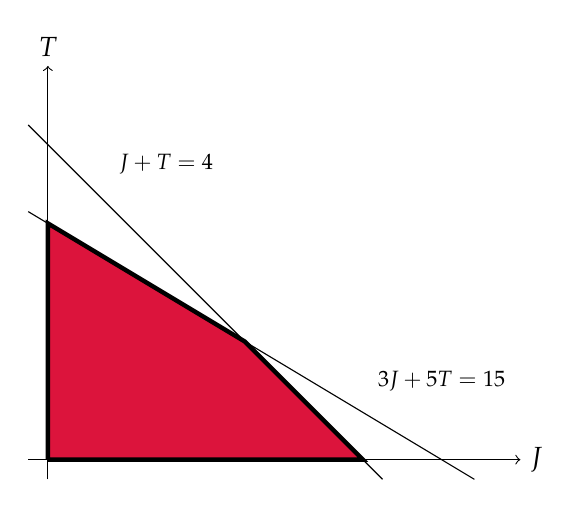
\begin{tikzpicture}
			\draw[->] (-0.25,0) -- (6,0) node[right] {$J$};
    		\draw[->] (0,-0.25) -- (0,5) node[above] {$T$};
			\draw (-0.25,4.25) -- (4.25,-0.25);
			\draw (-0.25,3.15) -- (5.416,-0.25);
			\draw[ultra thick, fill=Crimson] (0,0) -- (4,0) -- (2.5,1.5) -- (0,3) -- (0,0);
			\node at (1.5, 3.75) {{\footnotesize $J + T = 4$}};
			\node at (5, 1) {{\footnotesize $3J + 5T = 15$}};
		\end{tikzpicture}
	\end{center}
\end{ex}

Let's consider one of our constraint inequalities:
\begin{align*}
	a_{i1}x_1 + \cdots + a_{in}x_n \leq b_i.
\end{align*}
This can be compactly written as $a^{\top}x \leq b_i$ for $a\in\R^n$ and $b_i\in
\R$. The \emph{equation} 
\begin{align*}
	a^{\top}x = b_i 
\end{align*}
defines a \define{hyperplane} in $\R^n$: the vector $a$ describes the ``slope''
and the scalar $b_i$ describes how far the hyperplanes shifts away from the
origin. The hyperplane $a^{\top}x = b_i$ is the boundary of the set of solutions
to $a^{\top}x \leq b_i$. In $\R^2$, hyperplanes are lines, and in $\R^3$ they
are planes. 

\begin{figure}[h]
	\centering 
	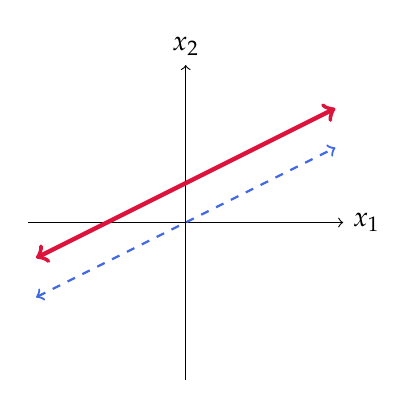
\begin{tikzpicture}
		\draw[->] (-2,0) -- (2,0) node[right] {$x_1$};
		\draw[->] (0,-2) -- (0,2) node[above] {$x_2$};
		\draw[<->, ultra thick, Crimson] (-1.9,-0.45) -- (1.9,1.45);
		\draw[<->, thick, RoyalBlue, dashed] (-1.9, -0.95) -- (1.9, 0.95);
	\end{tikzpicture}
	\caption{The line given by $a = (-1, 2)$, $b=1$ in red, and the line with $a = (-1, 2)$, $b=0$ is in blue.}
\end{figure}

Hyperplanes $H$ in $\R^n$ partition $\R^n$ into three sets: the points ``below''
$H$, the points ``above'' $H$, and the points on $H$. The set of points below
$H$ define a \define{half-space}, and similarly for the set of points above $H$. More precisely, if 
\begin{align*}
	H &= \{x\in \R^n \mid a^{\top}x = b\},
\end{align*}
then both 
\begin{align*}
	H^+ &= \{x\in \R^n \mid a^{\top}x > b \}, \\
	H^- &= \{x\in \R^n \mid a^{\top}x < b \}
\end{align*}
are half-spaces of $\R^n$. The \define{closed half-spaces} are 
\begin{align*}
	\overline{H^+} &= \{x\in \R^n \mid a^{\top}x \geq b \} = H^+ \cup H, \\
	\overline{H^-} &= \{x\in \R^n \mid a^{\top}x \leq b \} = H^- \cup H.
\end{align*}

\begin{ex}
	The sets 
	\begin{align*}
		X &= \{x\in \R^4 \mid -x_1 -4x_2 + \sin(1)x_3 \leq \pi \} \\
		Y &= \{y\in \R^4 \mid 7y_1 + 7y_2 + 7y_3 + 7y_4 = 2\}, \\
		Z &= \{z\in\R^4 \mid -8z_1 + 4z_2 - 2z_3 + z_4 > 0\}
	\end{align*}
	respectively define a closed half-space, hyperplane, and half-space in
	$\R^4$.
\end{ex}

What does this have to do with LPs?







\newpage

\bibliography{bibliography} 
\bibliographystyle{abbrv}

\end{document}